\documentclass[journal=jacsat,manuscript=article]{achemso}
\usepackage[version=3]{mhchem}
\usepackage[utf8]{inputenc}
\usepackage{anysize}
\usepackage{float}
\usepackage{graphicx}
\usepackage{siunitx}

% AUTHORS
\author{Cristina Ruiz}
\altaffiliation{Both authors have equally contributed}
\author{Álvaro Raya-Barón}
\altaffiliation{Both authors have equally contributed}
\author{Manuel A. Ortuño}
\affiliation[b]{Institute of Chemical Research of Catalonia (ICIQ), The Barcelona Institute of Science and Technology (BIST), Av. Països Catalans 16, 43007 Tarragona, Spain.}
\email{mortuno@iciq.es}
\author{Ignacio Fernández}
\email{ifernan@ual.es}
\affiliation[a]{Department of Chemistry and Physics, Research centre CIAIMBITAL, Ctra. Sacramento, s/n, 04120 Almería, Spain.}

%FALTAN LAS ABREVIATURAS Y PALABRAS CLAVE

% TITLE
\title{Accelerating role of deaggregation agents in lithium-catalysed hydrosilylation of carbonyl compounds} %Electronic supplementary information (ESI) available: Kinetic plots, NMR spectra, computational details, intermediate and transition state structures. See DOI: 10.1039/d0dt01540g

% MANUSCRIPT
\begin{document}
\maketitle

	% ABSTRACT
	
	\begin{abstract}
		% https://github.com/cristiruizblaze/proyecto_final{\tiny }
		
		A combined computational and experimental approach demonstrates the accelerating role of deaggregation agents, especially HMPA, in the Li-catalysed hydrosilylation of acetophenone in THF solution under very mild conditions.
	\end{abstract}
	
	% INTRODUCTION
	
	\section{Introduction}
	The reduction of carbonyl groups into alcohols is of wide interest in synthetic chemistry and therefore, constant efforts are	put into developing new efficient methodologies and perfecting the existing ones. Catalytic hydrosilylation1 has emerged as a convenient method as it operates under mild conditions and	combines an exceptional reducing capability with a high selectivity that can be finely tuned via catalyst design.
	
	% STATE OF THE ART
	
	\section{State of the art}
	Many Earth-abundant first-row transition metals, specially iron,2,3 have been tested in catalytic hydrosilylation of carbonyl compounds, as they are usually more environmentally-friendly and less toxic than their second- and third-row counterparts. Alkali metal salts have also been explored as alternative catalysts, initially by the groups of Corriu4 and Hosomi,5 and later by Beller6 and Nikonov,7 among others. Such compounds have been employed to promote hydrosilylation due to their basic character via formation of a pentacoordinated hydridosilicate,6–8 usually neglecting any relevant role of the alkali cation in the reaction mechanism. We recently reported	the hydrosilylation of carbonyl compounds catalysed by lithiated hydrazones.9 However, full understanding at atomic level of detail is still needed for the rational design of catalysts and reaction conditions.
	\\Herein we join computational and experimental efforts to understand and optimise processes catalysed by alkali–metal amides.10 Following theoretical guidance, we demonstrate how deaggregation agents (DAs) can efficiently accelerate hydrosilylation of carbonyl compounds in the presence of readily available lithium amides (Scheme 1) under very mild conditions such as room temperature and very low catalyst loading.
	\\

\renewcommand{\figurename}{Scheme}

	\begin{figure}[h]
	\includegraphics[width=0.6\textwidth]{figures/Síntesis.PNG}
	\centering
	\caption{Hydrosilylation of ketones catalysed by the combination of	Li-amides with deaggregation agents}
	\label{Scheme1}
	\end{figure}	

	% RESULTS AND DISCUSSION
	
	\section{Results and discussion}
	First, we computed the reaction mechanism for acetophenone and (MeO)2MeSiH using lithium diisopropylamide (LDA) as catalyst.9 The proposed reaction mechanism entails an activation step (Scheme 2a) prior to the catalytic cycle (Scheme 2b). We start from the LDA dimer 1 in THF solution. Dissociation of 111 via coordination of carbonyl and silane reactants yields the monomeric intermediates 2 and 3 at 17.8 kcal mol-1. The Si-H bond is then activated via amide nucleophilic attack,12 giving rise to a putative Li–hydride 5 as in Fe analogues 13,14 via -25 kcal mol-1. Although such transient intermediate would be very difficult to detect experimentally, similar species have been proposed in related literature. 15,16 Insertion of acetophenone into the Li-H bond generates an alkoxide 6 which activates a silane molecule 8 through a pentacoordinated hydridosilicate. Subsequent	hydride transfer releases the product and regenerates the Li-H species 5. According to the reaction profile (Scheme 2c), all relative activation Gibbs energies within the cycle are rather small, in the range of 7-10 kcal mol-1, with an overall value of 9.5 kcal mol-1 above 6. The most energy-demanding steps concern the initial dissociation of 1 to monomer 3 via 17.8 kcal mol-1 followed by the formation of hydride 5 via 25.4 kcal mol-1.
	
	\begin{center}
	\begin{minipage}{0.6\textwidth} 
		\begin{figure}[H]
			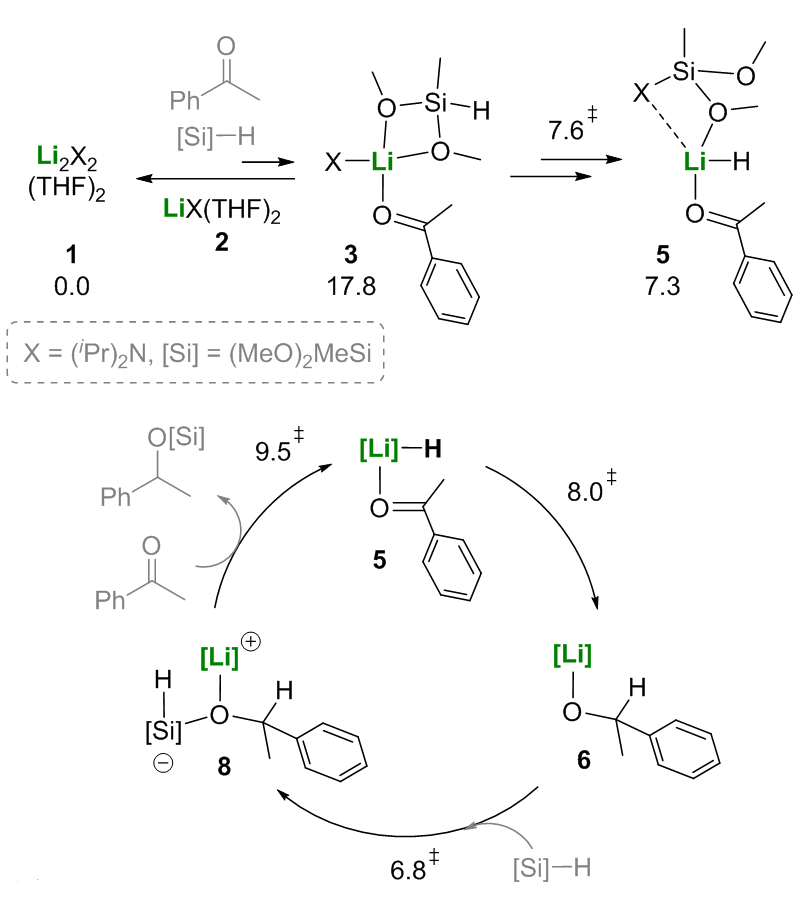
\includegraphics[width=\textwidth]{figures/Ciclo.PNG}
			\end{figure}
	\end{minipage}

	\begin{minipage}{0.6\textwidth} 
		\begin{figure}[H]
			\includegraphics[width=\textwidth]{figures/Energía.PNG}
			\caption{\label{Figure 1} Computed (a) pre-activation step and catalytic cycle, and (b) reaction profile for the hydride-mediated Li-catalysed hydrosilylation of acetophenone. All Gibbs energies are given in THF in kcal mol-1.}
		\end{figure}
	\end{minipage}
	\end{center}
	
	Figure 1 shows the optimised structures for the key transition states of the pre-activation step. The amide ligand performs a nucleophilic attack to the silicon atom through a reactant-like TS3–4; later, the hydride migrates from silicon to lithium	through the reactant-like TS4-5.
	\\
	We have also computed an alkoxy-silicate-mediated reaction mechanism in the absence of hydride intermediates (Scheme 3). After initial formation of the active species 3, the catalytic cycle continues with amide nucleophilic attack (4), hydrogen transfer (6), and O-Si bond formation to form intermediate 9. Final regeneration of species 3 releases the product. All steps within the cycle present larger activation Gibbs energies	(19–26 kcal mol-1) compared to those in the previous hydride-mediated pathway (7-10 kcal mol-1).
	
	\begin{figure}[H]
	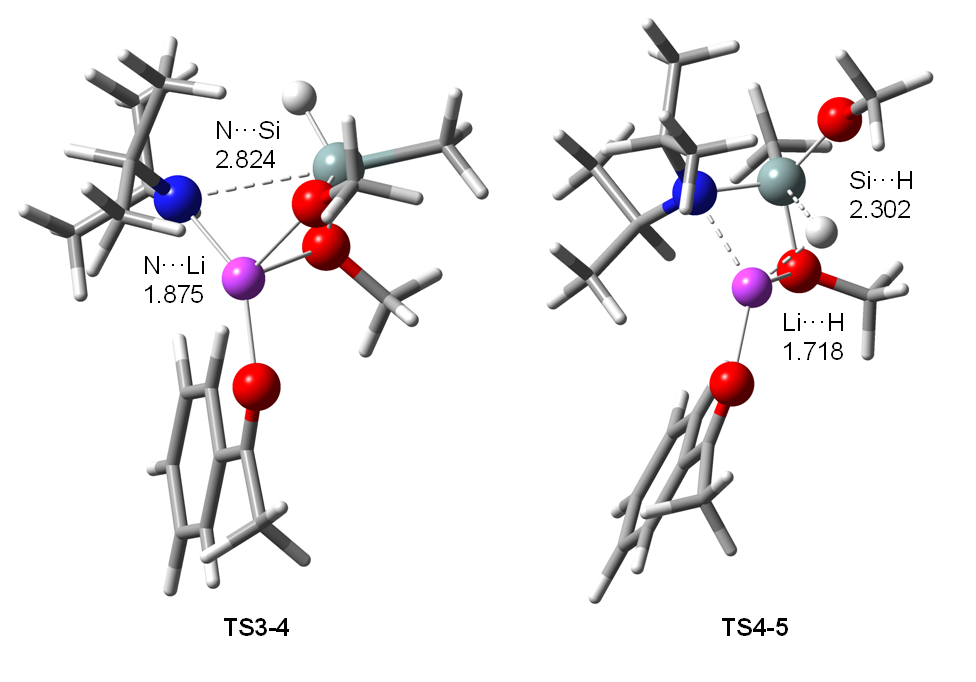
\includegraphics[width=0.5\textwidth]{figures/Nucleophilic attack.PNG}	
	\centering
	\caption{Optimised TS structures for nucleophilic attack (TS3-4) and hydride transfer (TS4-5). All distances in \si{\angstrom}.}
	\label{Figure1}
	\end{figure}	

	\begin{figure}[H]
	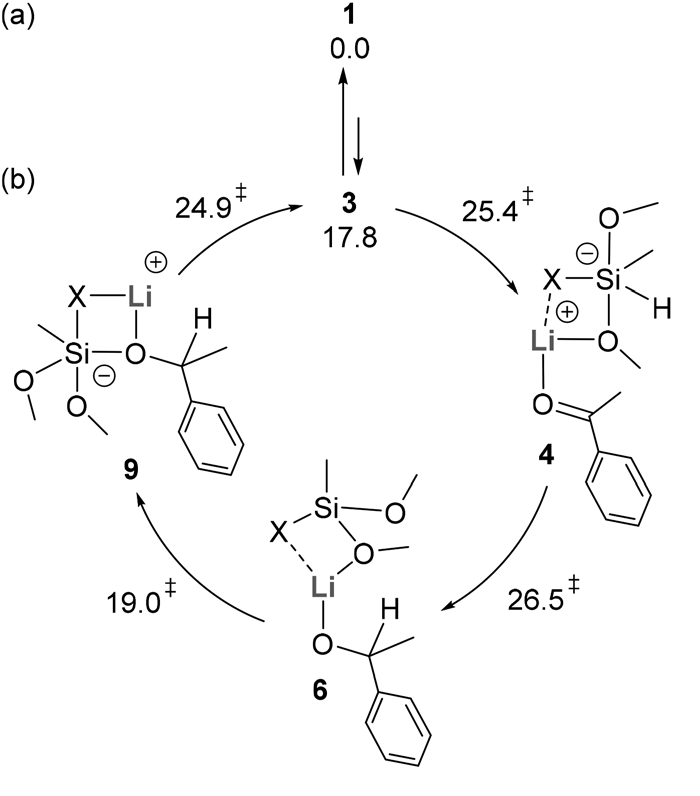
\includegraphics[width=0.4\textwidth]{figures/Cycle.PNG}		
	\centering
	\caption{Computed (a) pre-activation step and (b) catalytic cycle the alkoxy-silicate-mediated Li-catalysed hydrosilylation of acetophenone. All Gibbs energies are given in THF in kcal mol-1.}
	\label{Scheme 3}
	\end{figure}	

	Overall, the computational results suggest a rate-determining activation step to generate the catalytically active species 5, where a great part of the energy toll is related to the initial formation of a monomeric species 3 (Scheme 2a). We then envisage that using deaggregation agents (DAs)17 to displace the equilibrium towards monomeric species would entail a significant	increase in catalytic activity. DAs could also avoid oligomerization of other species such as 5 or 6. In a more general	way, the presence of DAs may favour or stabilise Li species	with lower levels of aggregations. 

	It is well documented how the reactivity of organolithium reagents shows significant solvent and co-solvent dependence.18 Most prominently, chelating N and O donor ligands such as pentamethyldiethylenetriamine (PMDTA), tetramethylethylenediamine 	(TMEDA), hexamethylphosphoramide (HMPA), and dimethylpropyleneurea (DMPU) are employed to deaggregate oligomeric s-ock organyls.19,20 Indeed, they can improve product yields, alter product distributions, and increase reaction rates through solvation and chelation of the metallic cations.21 Unfortunately, HMPA is a substance suspected	of carcinogenic potential in humans, and therefore appropriate safety procedures should be followed when handling this reagent in large-scale. 

	As a tentative approach to evaluate the impact of DAs on	reactivity, we have included one HMPA molecule during the
	rate-determining formation of the catalytically active species (Scheme 4). In species 1, HMPA displaces one THF; in species
	3, 4, and 5, it displaces the non-participating acetophenone. The computed Gibbs energies indicate that all intermediates
	are stabilised in the presence of HMPA. These results suggest a	better catalytic performance, either by facilitating the deaggregation of Li species (i.e., 17.8 kcal mol-1 from 1 to 3 vs. 12.6 kcal mol-1 from 1-DA to 3-DA) or by increasing the lifetime of key intermediates in solution (i.e., via the formation of 5-DA at 1.3 kcal mol-1). It is important to mention that the higher dielectric constant of HMPA, compared to THF, can have an impact on the computed energies when using continuum solvation models. Assuming that the amount of HMPA added to the solution is rather small (see later experiments),
	we expect similar energies for pure THF and HMPA-THF mixtures at our current level of theory.

	\begin{figure}[H]
	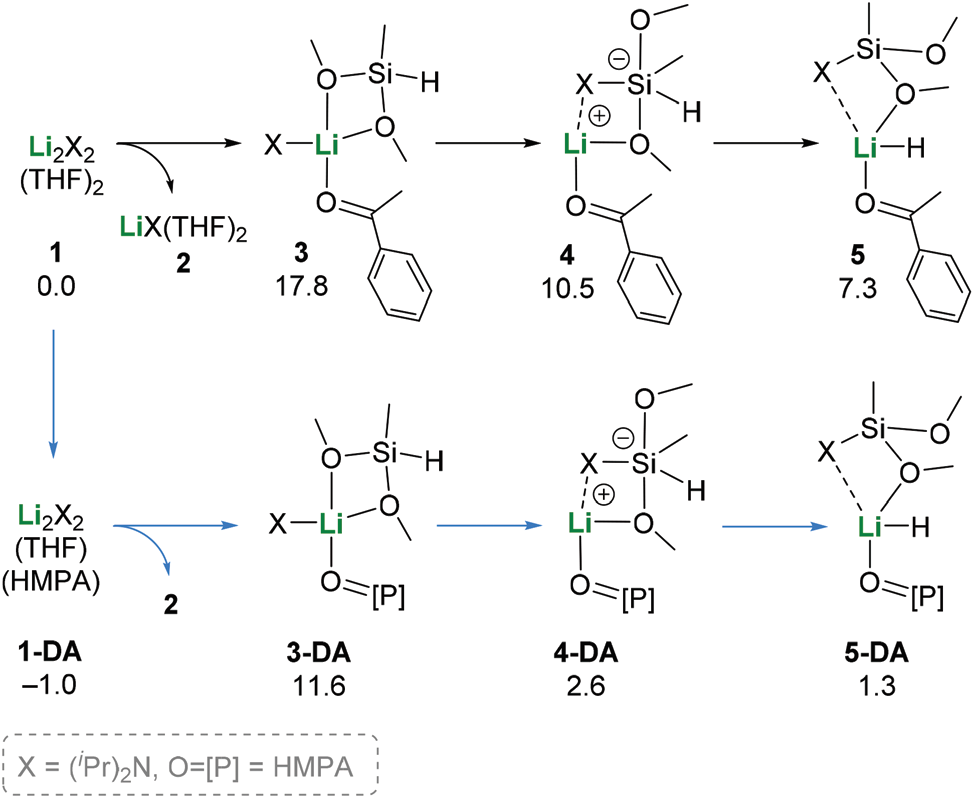
\includegraphics[width=0.6\textwidth]{figures/CompHMPA.PNG}		
	\centering
	\caption{Computed key intermediates in the presence of HMPA. All Gibbs energies are given in THF in kcal mol-1.}
	\label{Scheme4}
	\end{figure}

	To prove this hypothesis on Li-catalysed (0.25\% mol) hydrosilylations, we conducted a series of reactions catalysed by
	commercial amides (lithium diisopropylamide or LDA, lithium bis(trimethylsilyl) amide or LiHMDS, and lithium tetramethylpiperidide or LiTMP) as well as by the anthraquinoid lithium	hydrazone LiAQ,9 each of one in the presence (1.5\% mol, sixfold with respect to the catalyst) and the absence of DAs (Scheme 5 and Table 1). We firstly select HMPA as a representative example due to its commonly usage for this purpose.22 These catalytic runs were monitored via 1H NMR spectroscopy, which allowed us to detect initial rates, culmination steps and conversions (Fig. S1-7). The catalytic outcome remained the same when increasing the excess of HMPA up to 12-fold or 32-fold.
	
	\begin{figure}[H]
	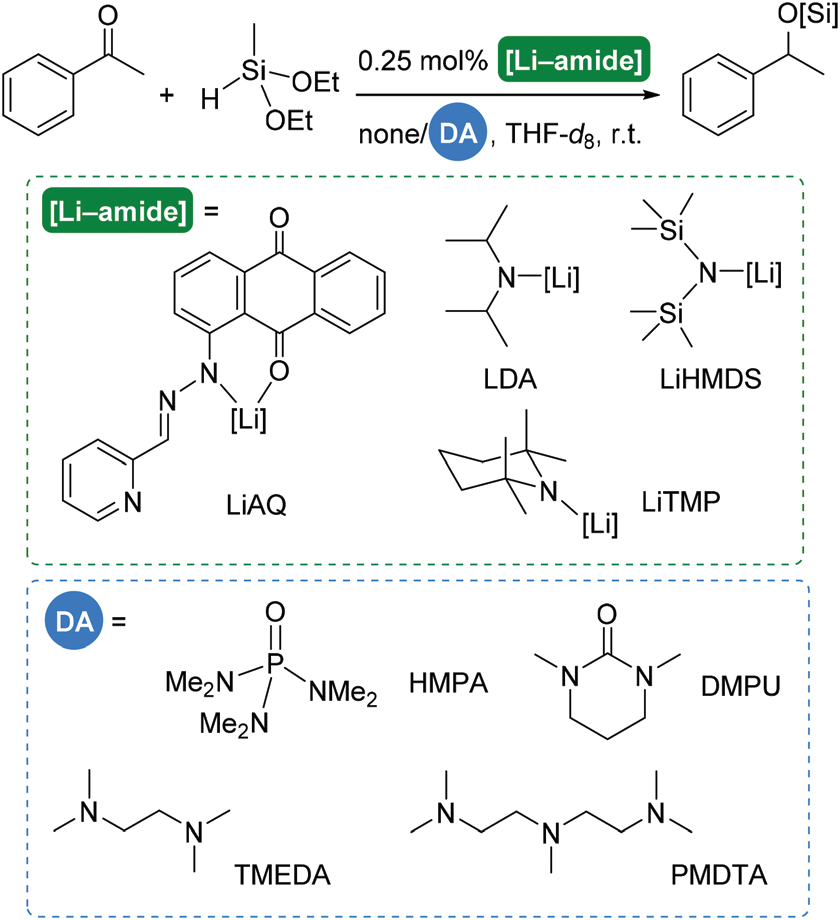
\includegraphics[width=0.6\textwidth]{figures/Reaction.PNG}		
	\centering
	\caption{Reaction conditions: acetophenone (1.0 mmol), (EtO)2MeSiH (1.1 mmol), Li-amide precursor (0.25 mol\%), deaggregation
		agent (none or 1.5 mol\%), THF-d8 (0.5 mL), 294 K.}
	\label{Scheme5}
	\end{figure}
	
	\begin{table}
		\caption{Turnover frequency (TOF) values obtained at different conversions for the hydrosilylation of acetophenone. LDA, LiHMDS, LiTMP, and LiAQ as catalysts and (EtO)2MeSiH as reducing agent}
		\begin{tabular}{|c|c|c|c}
			\hline
			Entry & Conditions a & TOF 30\%/min-1 & TOF 95\%/min-1 \\
			\hline
			1 & LDA & 11.4 & 2.1 \\
			\hline
			2 & LiAQ & 12.4 & 1.5 \\
			\hline
			3 & LiTMP & 12.2 & 1.4 \\
			\hline
			4 & LiHMDS & 14.7 & 2.2 \\
			\hline
			5 & LDA, HMPA & 45.3 & 19.1 \\
			\hline
			6 & LiAQ, HMPA & 56.4 & 1.9 \\
			\hline
			7 & LiTMP, HMPA & 82.4 & 7.9 \\
			\hline
			8 & LiHMDS, HMPA & 58.2 & 17.4 \\
			\hline
			9 & LiHMDS, DMPU & 27.4 & 2.5 \\
			\hline
			10 & LiHMDS, TMEDA & 28.0 & 2.0 \\
			\hline
			11 & LiHMDS, PMDTA & 18.0 & 2.1 \\
			\hline
		\end{tabular}
	\end{table}
		
	
	As shown by the turnover frequency (TOF) values calculated at two different conversion steps (Table 1) and the kinetic profiles (Fig. S1–7), the reaction rates increased in the presence of catalytic amounts of DA. We observed an enhanced performance	of 4–5 times at 30\% conversion and 8–9 times at 95\% conversion. Neither the catalytic runs in the absence nor the	presence of DA evidenced significant induction periods in their kinetic profiles. In addition, control experiments aimed
	to rule out the potential catalytic role of the neutral deaggregation agent alone were performed, resulting in absence of
	reaction.
	
	
	

\end{document}